\documentclass[12pt,letterpaper]{article}



%%
%% Required packages:
%%
\usepackage{etex}
\usepackage{amsmath}
\usepackage{amssymb}
\usepackage{amstext}
\usepackage{amsthm}
\usepackage{fancyhdr,fancybox}
\usepackage{mathrsfs} % need for \mathscr command
\usepackage{multicol}
\usepackage[normalem]{ulem}
%\usepackage{pictex,pictexplus}
% \usepackage{pictexwd}
\usepackage{rotating}
\usepackage{url}
\usepackage{xfrac}
\usepackage{booktabs}
\usepackage{color,soul}
\usepackage{comment}

\usepackage{hyperref}
\hypersetup{
    colorlinks=true,     % false: boxed links; true: colored links
    linkcolor=blue,      % color of internal links
    citecolor=blue,      % color of links to bibliography
    filecolor=blue,      % color of file links
    urlcolor=blue        % color of external links
}


\usepackage{tikz}
\usetikzlibrary{backgrounds,calc}

%%
%% Common formatting commands
%%
\setlength{\parindent}{0in}
\setlength{\textwidth}{7in}
\setlength{\evensidemargin}{-0.25in}
\setlength{\oddsidemargin}{-0.25in}
\setlength{\parskip}{.5\baselineskip}
\setlength{\topmargin}{-0.5in}
\setlength{\textheight}{9in}

%               Problem and Part
\newcounter{problemnumber}
\newcounter{partnumber}
\newcounter{subpartnumber}
\newcommand{\Problem}{%
  \refstepcounter{problemnumber}%
  \setcounter{partnumber}{0}%
  \setcounter{subpartnumber}{0}%
  \item[\makebox{\hfil\textbf{\theproblemnumber.}\hfil}]%
  }
\newcommand{\InProblem}[2][1.6]{%
  \refstepcounter{problemnumber}%
  \setcounter{partnumber}{0}%
  \setcounter{subpartnumber}{0}%
  \textbf{\theproblemnumber.}\ \ \parbox[t]{#1in}{#2}%
}
\newcommand{\InSmallProblem}[1]{\InProblem[1.05]{#1}}
\newcommand{\NoProblem}[1]{%
  \mbox{\hfil\textbf{#1}\hfil}%
  }
\newcommand{\UnProblem}{%
  \refstepcounter{problemnumber}%
  \setcounter{partnumber}{0}%
  \setcounter{subpartnumber}{0}%
  \mbox{\hfil\textbf{\theproblemnumber.}\hfil}%
  }
\newcommand{\InFlexProblem}[1]{%
  \refstepcounter{problemnumber}%
  \setcounter{partnumber}{0}%
  \setcounter{subpartnumber}{0}%
  \textbf{\theproblemnumber.}\ \ #1%
}
%%  Part:
\newcommand{\Part}{%
  \renewcommand{\thepartnumber}{(\alph{partnumber})}%
  \refstepcounter{partnumber}
  \setcounter{subpartnumber}{0}%
  \item[(\alph{partnumber})]%
}
\newcommand{\InPart}[2][1.75]{%
  \renewcommand{\thepartnumber}{(\alph{partnumber})}%
  \refstepcounter{partnumber}%
  \setcounter{subpartnumber}{0}%
  (\alph{partnumber})\ \ \parbox[t]{#1in}{#2}%
}
\newcommand{\UnPart}{%
  \refstepcounter{partnumber}%
  \renewcommand{\thepartnumber}{(\alph{partnumber})}%
  \setcounter{subpartnumber}{0}%
  (\alph{partnumber})%
}
\newcommand{\InLargePart}[1]{\InPart[3.05]{#1}}
\newcommand{\InFullPart}[1]{\InPart[6.2]{#1}}
\newcommand{\InSmallPart}[1]{\InPart[1.05]{#1}}
%% SubPart:
\newcommand{\SubPart}{%
  \refstepcounter{subpartnumber}%
  \item[(\roman{subpartnumber})]%
  }
\newcommand{\InSubPart}[2][2.25]{%
  \stepcounter{subpartnumber}%
  (\roman{subpartnumber})\ \ \parbox[t]{#1in}{#2}%
}
\newcommand{\InSmallSubPart}[1]{\InSubPart[1.5]{#1}}
\newcommand{\InTinySubPart}[1]{%
  \stepcounter{subpartnumber}%
  (\roman{subpartnumber})\ \ \makebox{#1}%
}
\newcommand{\InMySubPart}[2][2.25]{%
  \stepcounter{subpartnumber}%
  \parbox[t]{#1in}{\makebox[0.3in][l]{(\roman{subpartnumber})}\ \ {#2}}%
}
\newcommand{\TrueFalse}{\textbf{T}\ \ \textbf{F}\ \ }
\newcommand{\TFPart}[1]{% 
  \stepcounter{partnumber}%
  \setcounter{subpartnumber}{0}%
  \item[(\alph{partnumber})] \TrueFalse\parbox[t]{5.5in}{#1}}

\newcommand{\Points}[1]{(#1 points) \ }
\newcommand{\Point}[1]{(#1 point) \ }


%% For Answers:
\newcounter{answernumber}
\newcommand{\Answer}{%
  \refstepcounter{answernumber}%
  \setcounter{partnumber}{0}%
  \setcounter{subpartnumber}{0}%
  \item[\makebox{\hfil\textbf{\theanswernumber.}\hfil}]%
  }


% Setting up the headers for the first page
%\chead{} % will default to what is typed in the file.
\fancyhead[L]{\textsc{Math 22a}}
\fancyhead[R]{\textsc{Fall 2024}}
\fancyfoot[R]{
	\vspace*{\fill}\footnotesize\textcopyright{} \emph{Harvard Math 22a}	
}
\renewcommand{\headrulewidth}{0pt}

%\fancyhead[C]{}
%	\chead{}	
%	\lhead{}
%	\rhead{}
%	\cfoot{}


% Putting copyright on the footer of each page
%\fancypagestyle{secondpage}{
%	\fancyhead[C]{TESTing again} % change this to be blank
%		%\chead{}	
%	\fancyhead[L]{bears} % change this to be blank
%	\fancyhead[R]{dogs} % change this to be blank
%	\fancyfoot[R]{ %keeps the footer the same
%		\vspace*{\fill}\footnotesize\textcopyright{} \emph{Harvard Math 22a}	
%	}
%}
%\renewcommand{\headrulewidth}{0pt}
%\pagestyle{fancy}
\pagestyle{empty}


%\lhead{}
%\rhead{}
%\rfoot{\vspace*{\fill}\footnotesize\textcopyright{} \emph{Harvard Math 22a}}
%\renewcommand{\headrulewidth}{0pt}
%\pagestyle{fancy}




%%
%% Common shortcut commands:
%%
\newcommand{\ds}{\displaystyle}
\newcommand{\sgn}{\operatorname{sgn}}
\renewcommand{\Pr}{\operatorname{P}}
\newcommand{\CPr}[3][{}]{\Pr_{\text{#1}}\left(#2\,|\,#3\right)}

\newcommand{\C}{\mathbb{C}}
\newcommand{\R}{\mathbb{R}}
\newcommand{\Z}{\mathbb{Z}}
\newcommand{\N}{\mathbb{N}}
\newcommand{\Q}{\mathbb{Q}}
\newcommand{\D}{\mathbb{D}}

\newcommand{\rref}{\operatorname{rref}}
\newcommand{\im}{\operatorname{im}}
\newcommand{\rank}{\operatorname{rank}}
\newcommand{\diag}{\operatorname{diag}}
\newcommand{\Span}{\operatorname{span}}
%\renewcommand{\vec}[1]{\mathbf{#1}}
\newcommand{\charpoly}{\mathscr{P}}
\newcommand{\nicefrac}[2]{\sfrac{#1}{#2}} % using xfrac package
\newcommand{\topology}{\mathcal{T}}
\newcommand{\Inn}{\operatorname{Inn}}

\newcommand{\blankbox}[2]{\fbox{\rule{#1}{0in}\rule{0in}{#2}}}

\newenvironment{myindentpar}[1]%
 {\begin{list}{}%
         {\setlength{\leftmargin}{#1}
          \setlength{\rightmargin}{\leftmargin}}%
         \item[]%
 }
 {\end{list}}
\newtheorem{theorem}{Theorem}
\newtheorem*{NStheorem}{Theorem}
\newtheorem{cor}[theorem]{Corollary}
\newtheorem*{claim}{Claim}
\newtheorem{defn}{Definition}

\newenvironment{amatrix}[1]{%
  \left(\begin{array}{@{}*{#1}{c}|c@{}}
}{%
  \end{array}\right)
}

%--------grstep
% For denoting a Gauss' reduction step.
% Use as: \grstep{\rho_1+\rho_3} or \grstep[2\rho_5 \\ 3\rho_6]{\rho_1+\rho_3}
\newcommand{\grstep}[2][\relax]{%
   \ensuremath{\mathrel{
       {\mathop{\longrightarrow}\limits^{#2\mathstrut}_{
                                     \begin{subarray}{l} #1 \end{subarray}}}}}}
\newcommand{\swap}{\leftrightarrow}


\usetikzlibrary{arrows}
\usepackage{wrapfig}
\usepackage{amsfonts}

\makeatletter
\renewcommand*\env@matrix[1][*\c@MaxMatrixCols c]{%
	\hskip -\arraycolsep
	\let\@ifnextchar\new@ifnextchar
	\array{#1}}
\makeatother

\def\env@matrix{\hskip -\arraycolsep
	\let\@ifnextchar\new@ifnextchar
	\array{*\c@MaxMatrixCols c}}

\chead{\Large\textbf{Differential Equations, $\vec\S$5.6, 5.7}}% 

\begin{document}
\thispagestyle{fancy}

Recall from previously:

\begin{itemize}
\item If $A$ is an $n \times n$ matrix, then $\lambda \in \mathbb{R}$ is an {\bf eigenvalue} of $A$ if there exists a non-zero vector $v$, called an {\bf eigenvector} corresponding to $\lambda$, such that $$Av=\lambda v.$$
\item If $\lambda$ is an eigenvalue of an $n \times n$ matrix $A$, then the set of all solutions $v$ to $Av = \lambda v$ is the {\bf eigenspace} of $A$ corresponding to $\lambda$.
\item {\bf Theorem 1:} The eigenvalues of a triangular matrix are the diagonal entries.
\item {\bf Theorem 2:} If $v_1, \dots, v_p$ are eigenvectors corresponding to distinct eigenvalues $\lambda_1, \dots, \lambda_p$ of an $n\times n$ matrix $A$, then $v_1, \dots, v_p$ are linearly independent.
\item If $A$ is an $n\times n$ matrix, then the characteristic polynomial of $A$, denoted by $p_A(\lambda)$, is given by $$p_A(\lambda)=\text{det}(A-\lambda I_n).$$
\item $\lambda$ is an eigenvalue of an $n\times n$ matrix $A$ if and only if $\lambda$ is a zero of the characteristic polynomial.
\item If $A$ and $B$ are similar matrices, then they have the same characteristic polynomials and hence the same eigenvalues (with the same algebraic multiplicities). 
\item An $n\times n$ matrix $A$ is {\bf diagonalizable} if $A$ is similar to a diagonal matrix.
\item {\bf Diagonalization Theorem:} An $n \times n$ matrix $A$ is diagonalizable if and only if $A$ has $n$ linearly independent eigenvectors. Moreover, $A=PDP^{-1}$ with $D$ diagonal if and only if the columns of $P$ are $n$ linearly independent eigenvectors of $A$. In this case the diagonal entires of $D$ are the corresponding eigenvalues of $A$.
\item {\bf Theorem 6:} An $n \times n$ matrix $A$ with $n$ distinct eigenvalues is diagonalizable.
\item 
{\bf Theorem 7:} Let $A$ be an $n\times n$ matrix with distinct eigenvalues $\lambda_1, \dots, \lambda_p$.
\begin{enumerate}
\item For $1\leq k \leq p$, the dimension of the eigenspace of $\lambda_k$ is at most the algebraic multiplicity of the eigenvalue $\lambda_k$.
\item The matrix $A$ is diagonalizable if and only if the sum of the dimensions of the eigenspaces is $n$ if and only if the characteristic polynomial factors into linear factors and the dimension for each eigenspace is exactly the algebraic multiplicity.
\item If $A$ is diagonalizable and $\mathcal{B}_k$ is a basis for the eigenspace corresponding to $\lambda_k$, then $\mathcal{B}_1, \dots, \mathcal{B}_p$ is an eigenbasis for $\mathbb{R}^n$.
\end{enumerate}
\end{itemize}

\newpage


\begin{enumerate}

\Problem Recall the differential equation $y''(t) = -y(t)$ as modeling a unit mass on a spring. Solve the differential equation.

\newpage

\Problem Consider $x'(t) = \begin{bmatrix} 1 & 2\\ 3 & 2\\ \end{bmatrix} x(t)$. Solve the differential equation.

\vfill

\Problem Consider $x'(t) = \begin{bmatrix} 0 & -1\\ 1 & 0\\ \end{bmatrix} x(t)$. Solve the differential equation.

\vfill


\newpage


\end{enumerate}

\begin{comment}
\newpage
\chead{\Large\textbf{Differential Equations -- Answers / Solutions}}%
\lhead{}
\rhead{}
\thispagestyle{fancy}

\begin{enumerate}
\Answer Recall we solve second order constant coefficient differential equations by guessing a solution of the form $y(t)=e^{rt}$ for $r$ is a constant. Plugging in to the differential equation we get $$(r^2+1)e^{rt}=0,$$ and hence $r^2+1=0$. Thus we get solutions when $r=\pm i$. Thus we get two independent solutions $e^{it}$ and $e^{-it}$. The general solution is then $$y(t)= c_1 e^{it}+c_2 e^{-it}.$$ We call this the complex form of the general solution. Instead we might prefer to have a real form for the solutions. Using $e^{it}=\cos{t}+i\sin{t}$, we get $$y(t)=c_1(\cos{t}+i\sin{t}) +c_2 (\cos{t}-i \sin{t})= (c_1+c_2)\cos{t}+i(c_1-c_2)\sin{t}.$$ Now notice that the real and imaginary parts of $(c_1+c_2)\cos{t}+i(c_1-c_2)\sin{t}$ are themselves solutions to the differential equation, and hence we get the real form of the general solution is $$y(t)= d_1 \cos{t} +d_2 \sin{t}.$$

On the other hand we can let $v(t)=y'(t)$, then we get the system of first order equations $$\begin{cases} v'(t) = -y(t)& \\ y'(t)=v(t),&\end{cases} $$ or $$\begin{bmatrix} v(t)\\ y(t)\\ \end{bmatrix}' = \begin{bmatrix} 0 & -1 \\ 1 & 0 \\ \end{bmatrix}\begin{bmatrix} v(t)\\ y(t)\\ \end{bmatrix}=A\begin{bmatrix} v(t)\\ y(t)\\ \end{bmatrix}.$$

Thus we want to solve the system $$\vec{y}\prime(t)= A \vec{y}.$$ We guess a solution of the form $y(t)= \vec{v} e^{\lambda t}$ and we get $$\vec{v}\lambda e^{\lambda t} = A \vec{v} e^{\lambda t},$$ or $$(A\vec{v}-\lambda \vec{v})e^{\lambda t} =0.$$ Thus $y(t)$ is a solution if and only if $A\vec{v}=\lambda \vec{v}$. Thus $\vec{v}$ must be an eigenvector with eigenvalue $\lambda$. Thus we get the complex form of the general solution by using the eigenvalues and eigenvectors; namely, $$y(t)= c_1 \vec{v}_1 e^{\lambda_1 t} + c_2 \vec{v}_2 e^{\lambda_2 t}.$$ Plugging in the eigenvalues and eigenvectors for $A$ we get $$\vec{y}(t)= c_1\begin{bmatrix} 1\\ -i\\ \end{bmatrix} e^{i t} + c_2 \begin{bmatrix} 1\\ i\\ \end{bmatrix} e^{-it},$$ and hence $$y(t)= c_1(- i) e^{it} +c_2 ie^{-it}.$$ We can again use Euler's formula to get the real-form of the solution. Here we take the real and imaginary parts of $\begin{bmatrix} 1\\ -i\\ \end{bmatrix} e^{i t}$ to get $$\left(\begin{bmatrix} 1\\ 0\\ \end{bmatrix}+i\begin{bmatrix} 0\\ -1\\ \end{bmatrix}\right)(\cos{t}+i\sin{t})= \left(\begin{bmatrix} 1\\ 0\\ \end{bmatrix} \cos{t} - \begin{bmatrix} 0\\ -1\\ \end{bmatrix} \sin{t}\right)+i \left(\begin{bmatrix} 1\\ 0\\ \end{bmatrix} \sin{t}+\begin{bmatrix} 0\\ -1\\ \end{bmatrix} \cos{t}\right).$$ Again the real and imaginary parts are separately solutions to the differential equations, and hence we get the real form of the general solution is given by $$\vec{y}(t)= d_1 \begin{bmatrix} \cos{t}\\ \sin{t} \end{bmatrix}+d_2 \begin{bmatrix} \sin{t}\\ -\cos{t}\\ \end{bmatrix}.$$ Thus when $d_1=1$ and $d_2=0$ we get a circle of radius one in the phase portrait as shown below.

\begin{center}
	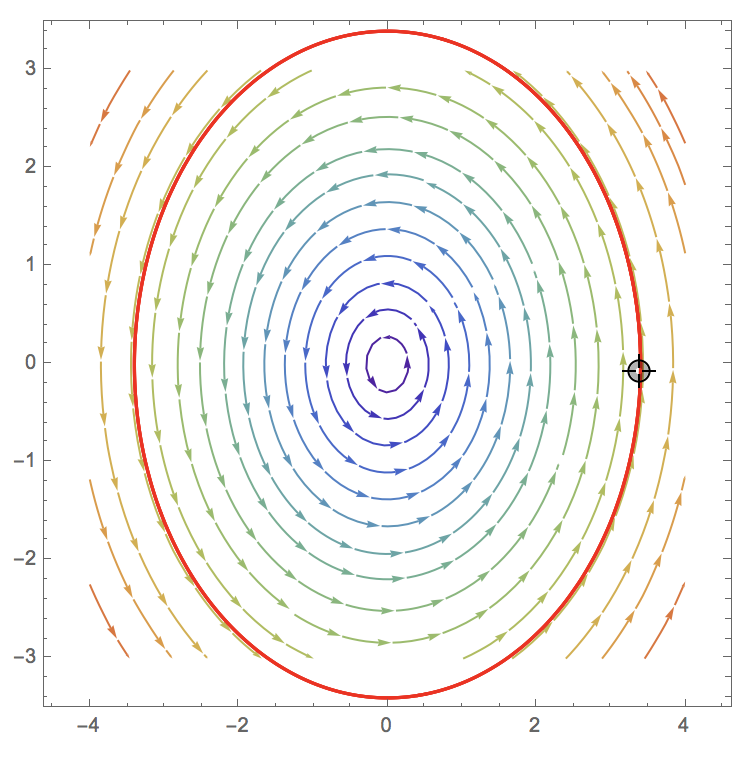
\includegraphics{phase2.png}
\end{center}

\Answer We again find eigenvalues and eigenvectors. Here we get eigenvalues of $4$ and $-1$. The eigenspaces are given by $$E_{-1}=\text{Span}\left\{\begin{bmatrix} -1\\ 1\\ \end{bmatrix}\right\},$$ and $$E_{4}=\text{Span}\left\{\begin{bmatrix} 2\\ 3\\ \end{bmatrix}\right\}.$$ Then the general solution is given by $$\vec{x}(t)= c_1 \begin{bmatrix} 2\\ 3\\ \end{bmatrix} e^{4t} +c_2 \begin{bmatrix} -1\\ 1\\ \end{bmatrix} e^{-t}.$$ We show the phase portrait with one solution trajectory in red below.

\begin{center}
	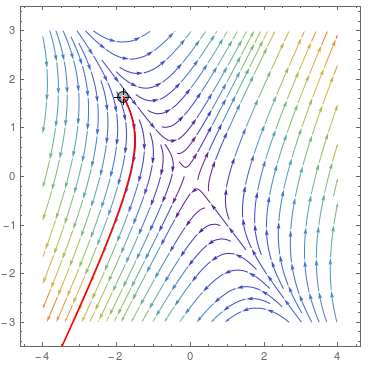
\includegraphics{phase4.png}
\end{center}
\Answer See the solution to question 1.

\end{enumerate}  

\end{comment}

\end{document}


%%% Local ables: 
%%% mode: latex
%%% TeX-master: t
%%% End: 
